\documentclass[10pt,a4paper]{article}
\usepackage[a4paper,top=15mm,bottom=15mm,left=16.5mm,right=16.5mm,headheight=14pt]{geometry}
\usepackage{fontspec}
\setsansfont{Arial}
\renewcommand{\familydefault}{\sfdefault}
\usepackage{graphicx}
\usepackage{booktabs,tabularx,array,longtable}
\usepackage{xcolor}
\usepackage{enumitem}
\usepackage{titlesec}
\usepackage{fancyhdr}
\usepackage{microtype}
\usepackage{hyperref}
\usepackage{caption}
\usepackage{float}
\usepackage{ragged2e}
\definecolor{navy}{HTML}{17365D}
\definecolor{blue}{HTML}{2F75B5}
\definecolor{paleblue}{HTML}{EEF5FB}
\definecolor{lightblue}{HTML}{DDEBF7}
\definecolor{graytext}{HTML}{666666}
\definecolor{rednote}{HTML}{C00000}
\hypersetup{colorlinks=true,linkcolor=navy,urlcolor=blue}
\pagestyle{fancy}
\fancyhf{}
\lhead{\footnotesize\color{graytext}Mode-I adaptive remeshing supervisor report}
\rfoot{\footnotesize\color{graytext}Page \thepage}
\renewcommand{\headrulewidth}{0pt}
\renewcommand{\footrulewidth}{0pt}
\titleformat{\section}{\Large\bfseries\color{black}}{}{0pt}{}
\titleformat{\subsection}{\large\bfseries\color{black}}{}{0pt}{}
\titlespacing*{\section}{0pt}{0pt}{6pt}
\titlespacing*{\subsection}{0pt}{5pt}{4pt}
\setlength{\parindent}{0pt}
\setlength{\parskip}{4pt}
\setlist[itemize]{leftmargin=5mm,itemsep=2pt,topsep=2pt}
\captionsetup{font={small,it},labelfont=bf,skip=3pt}
\newcolumntype{Y}{>{\RaggedRight\arraybackslash}X}
\newcommand{\rowcolor}[1]{}
\newcommand{\headrow}{\color{navy}\bfseries}
\newcommand{\src}[1]{\par{\footnotesize\color{graytext}\textbf{Source:} #1}}
\graphicspath{{figures/}}

\begin{document}
\thispagestyle{empty}
\vspace*{25mm}
\begin{center}
{\fontsize{22}{27}\selectfont\bfseries Application of Built in Adaptive Remeshing and Mesh Refinement Features in Abaqus to Phase Field Fracture Simulations\par}
\vspace{12mm}
{\fontsize{18}{22}\selectfont\bfseries\color{navy}Mode I Supervisor Report\par}
\vspace{8mm}
{\large 17 September 2026\par}
\vfill
{\large Pruthviraja Reddy Vandavagali\par}
\vspace{2mm}
Master Thesis in Computational Materials Science\par
Chair of Applied Mechanics IMFD\par
TU Bergakademie Freiberg\par
\vspace{20mm}
\end{center}

\newpage
\section{Executive Summary}
The Mode-I benchmark reconstruction now has a verified fixed-mesh response anchor, a verified Abaqus-native pre-refinement workflow, and a causally resolved preprocessing defect. The remaining scientific question is the adaptive mesh count: the canonical project rule with \texttt{errorTarget=1.0} produces 71,320 finite elements, whereas Pandey and Kumar report 13,941 for their proposed adaptive mesh.

\textbf{Important distinction between the two reported element counts.} The 26,282-element mesh and the 13,941-element mesh do not represent the mesh before and after one adaptive-remeshing operation. They belong to two separate simulations. In the \textbf{standard PFM}, a manually refined crack-propagation corridor with $h=0.003$ mm is embedded in a global $h=0.02$ mm mesh, resulting in 26,282 finite elements. In the \textbf{proposed adaptive PFM}, the analysis starts again from a separate coarse mesh with global $h=0.02$ mm and no equivalent manually pre-refined corridor. MISESERI then drives native adaptive remeshing to a final mesh of approximately 13,941 elements with local $h=0.001$ mm. The paper does not report the initial coarse element count for this adaptive route.

\small
\par\smallskip\noindent
\begin{tabularx}{\textwidth}{>{\bfseries}p{37mm}p{38mm}Y}
\headrow Result & Verified value & Scientific meaning\\
Published standard PFM & 26,282 elements & Global $h=0.02$ mm plus manual $h=0.003$ mm crack corridor\\
\rowcolor{paleblue}Published proposed adaptive PFM & 13,941 elements & Separate coarse branch; initial count not reported; local $h=0.001$ mm after remeshing\\
Project adaptive reconstruction & 2,906 $\rightarrow$ 71,320 & Canonical project pre-analysis and \texttt{errorTarget=1.0}\\
\rowcolor{paleblue}Fixed response anchor 1398090 & $F_{\max}=0.757778$ kN & Close agreement with the published Mode-I force-displacement response\\
Corrected nominal 1\% 1404933 & $K_0=137.820804$ kN/mm & Stiffness recovered after the \texttt{N\_BOTTOM} repair\\
\end{tabularx}\par\smallskip
\normalsize

The reduction from 26,282 to 13,941 must not be interpreted as adaptive remeshing reducing the element count. The correct comparison is between two alternative meshing strategies. For the 
\texttt{RemeshingRule} used in this study, coarsening is disabled (\texttt{coarseningFactor=NOT\_ALLOWED}); therefore the adaptive-remeshing operation is expected to increase, rather than decrease, the finite-element count relative to that adaptive route's own initial coarse mesh.
\src{Pandey and Kumar (2025), Sections 3.3 and 4.1; project Jobs 1398090, 1399632 and 1404933.}

\newpage
\section{Mode I Benchmark and Quantitative Reference}
The benchmark is a $1.0\times1.0$ mm square plate with a zero-gap horizontal crack of length $a_0=0.5$ mm along $y=0.5$ mm. The publication specifies vertical Mode-I loading and lower-edge support. The single $u_x=0$ restraint shown below removes rigid-body motion. A top-edge $U_1=0$ condition is a project reconstruction choice and is not presented as a published condition.
\begin{figure}[H]
\centering
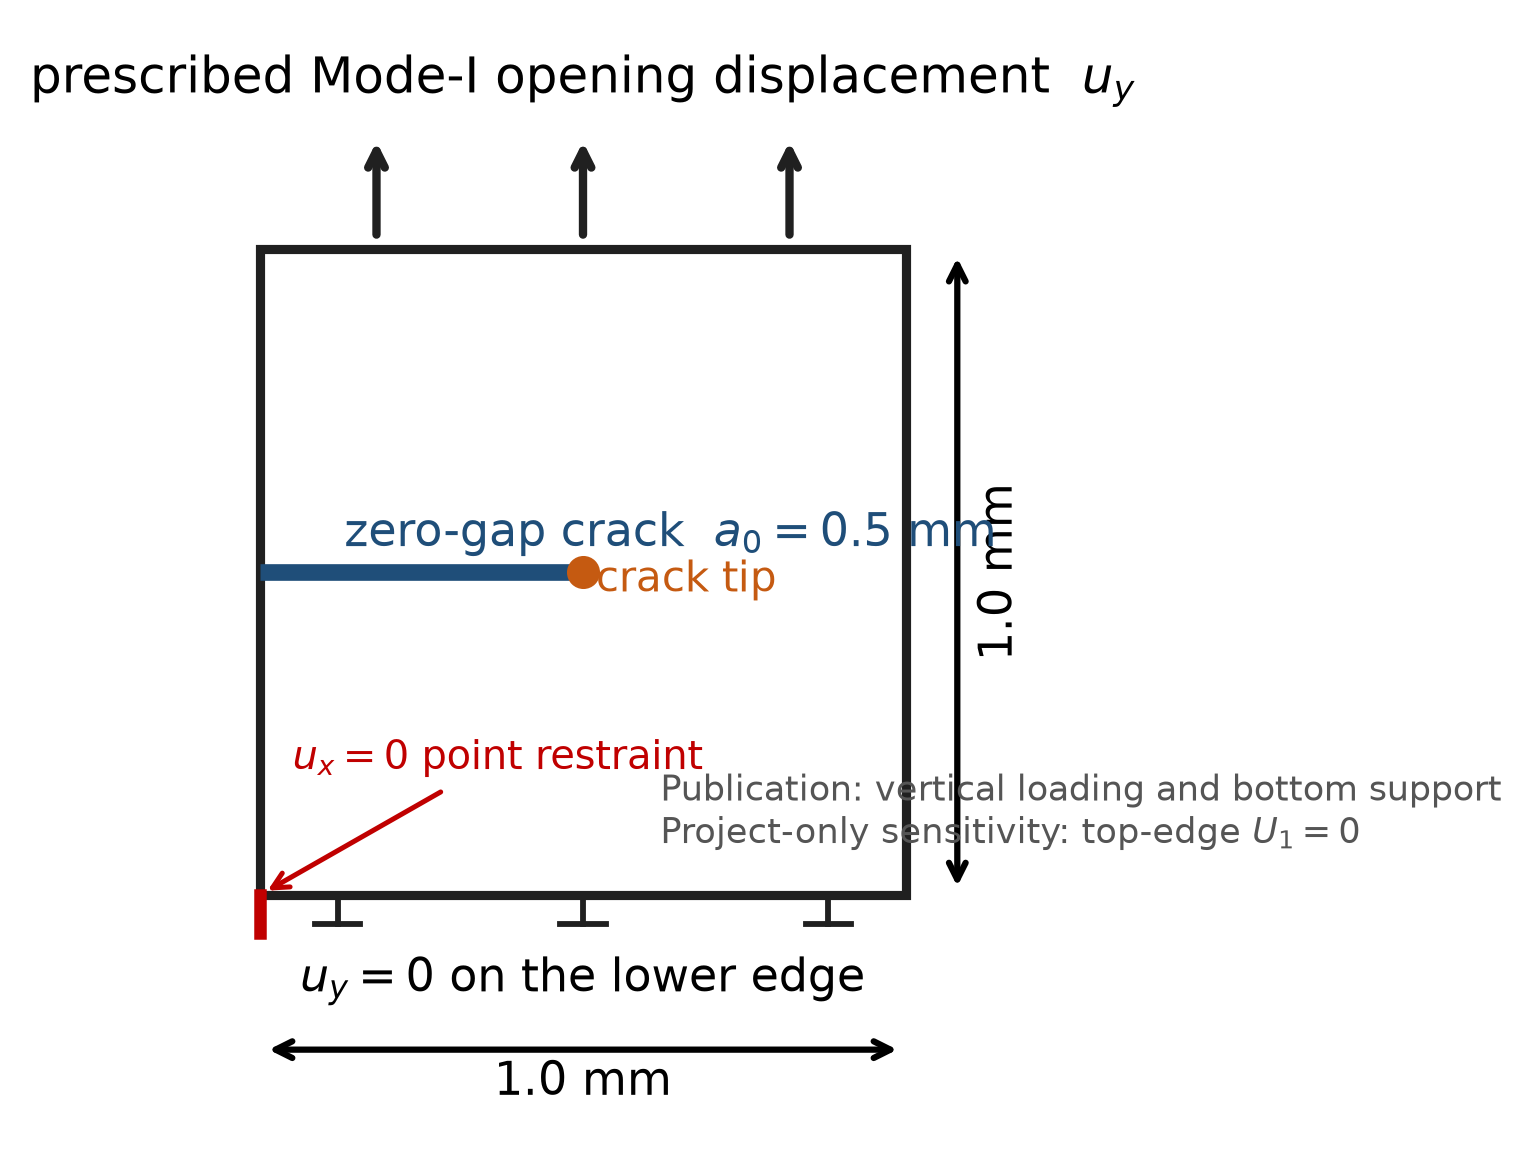
\includegraphics[width=0.82\textwidth,height=55mm,keepaspectratio]{mode1_geometry.png}
\caption{Mode-I geometry, crack, loading and boundary-condition provenance.}
\end{figure}
\vspace{-2mm}
\begin{figure}[H]
\centering
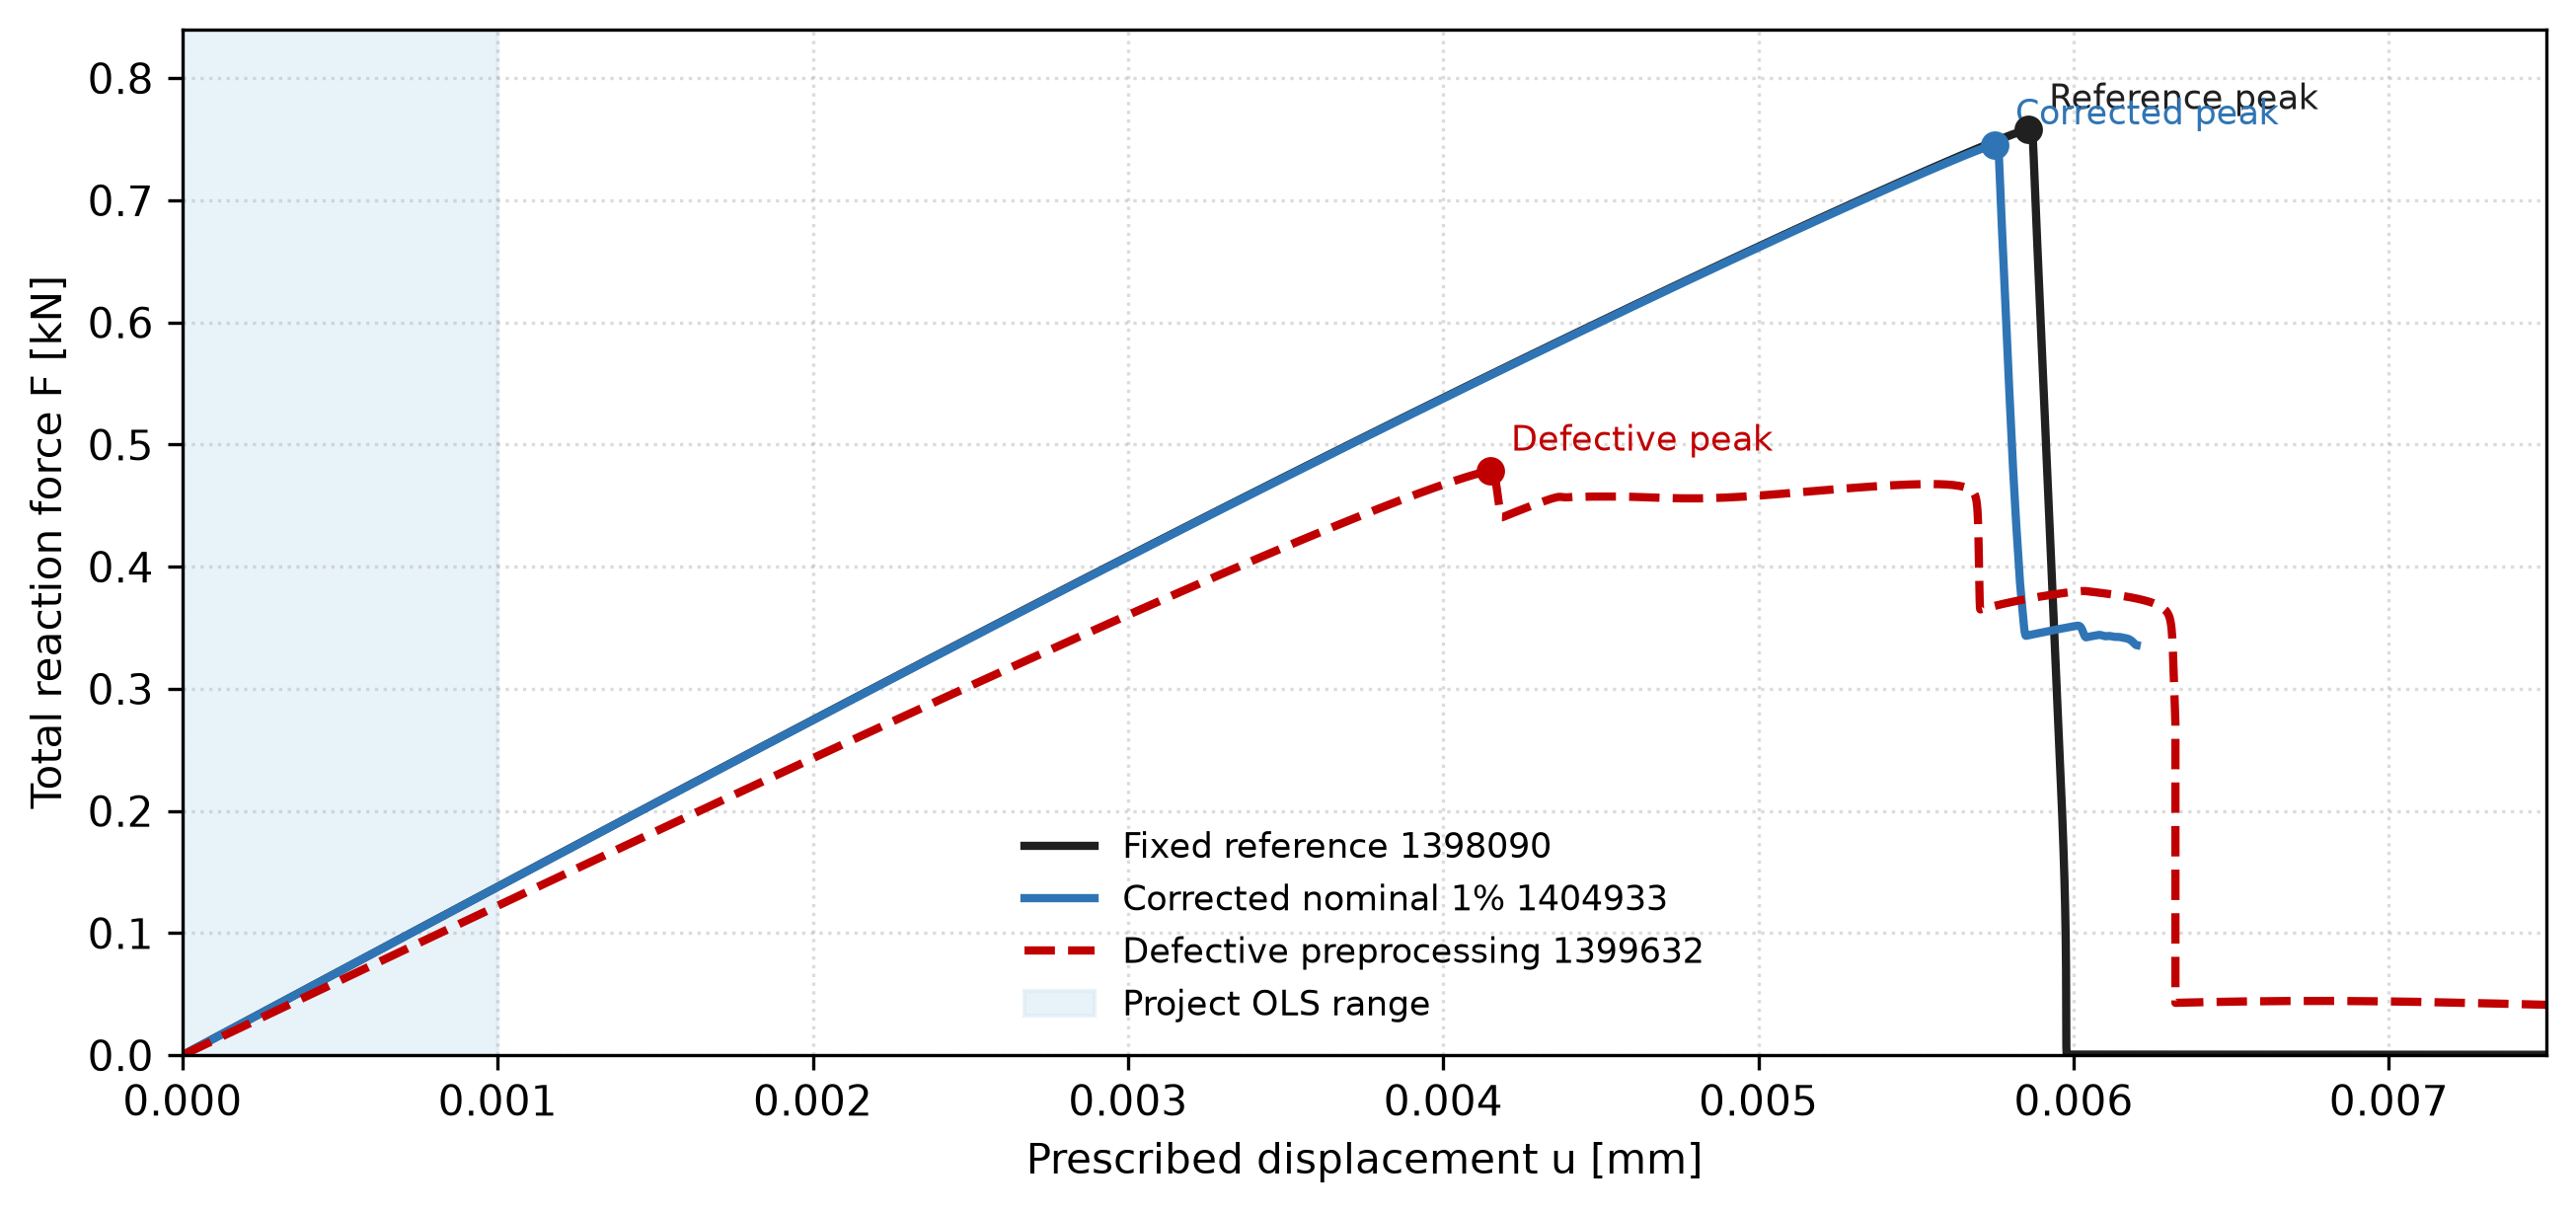
\includegraphics[width=0.93\textwidth,height=91mm,keepaspectratio]{force_displacement_full.png}
\caption{Full force-displacement comparison. Markers identify each peak; shading shows the project OLS range.}
\end{figure}
\vspace{-2mm}
{\small\textbf{Published comparison:} Pandey and Kumar (2025), Section 4.1 and Figure 7(a), support comparison of the force-displacement response. \textbf{Project-derived quantity:} $K_0=137.945520$ kN/mm is obtained from Job 1398090 by an OLS fit over the first 400 active increments; it is not a stiffness value reported by Pandey and Kumar.}

\newpage
\section{Multifaceted Mesh-Convergence Assessment}
\textbf{Peak load alone is not sufficient to demonstrate mesh convergence in a phase-field fracture model.} Mesh adequacy is therefore evaluated using complementary global and spatial quantities: the complete force--displacement response, initial structural stiffness, peak force and displacement at peak, external work over a common displacement interval, phase-field distribution, and crack-path/localization behaviour. Agreement across these measures provides a substantially stronger convergence assessment than comparison of $F_{\max}$ alone.

\scriptsize
\renewcommand{\arraystretch}{1.08}
\par\smallskip\noindent
\begin{tabularx}{\textwidth}{>{\bfseries}p{34mm}p{28mm}p{44mm}Y}
\headrow Quantity & Symbol / Range & Physical / Numerical Role & Observed Convergence Behaviour\\
Complete $F$--$u$ response & $F(u)$, $u \ge 0$ & Global structural and softening response & Not claimed: four refined-job raw curve files are not preserved in the report package\\
Initial stiffness $K_0$ & $K_0 = \left.\frac{\mathrm{d}F}{\mathrm{d}u}\right|_{u \le 1\,\mu\mathrm{m}}$ & Elastic compliance before damage onset & Invariant: $137.95 \to 137.82$ kN/mm ($0.089\%$ shift across $4.56\times$ FE count)\\
Peak force $F_{\max}$ & $F_{\max} = \max_u F(u)$ & Regularized structural fracture load & Monotonic decrease; successive changes generally reduce, but strict asymptotic convergence is not established\\
Displacement at peak & $u(F_{\max})$ & Deformation threshold for crack initiation & Monotonic decrease: $5.857 \to 5.575\,\mu$m; measurable mesh sensitivity remains\\
External work $W_{\mathrm{ext}}$ & $\int_0^{u_{\mathrm{common}}} F\,\mathrm{d}u$ & Global mechanical work from the $F$--$u$ response & Monotonic decrease: $2.3583 \to 2.1475$ mJ at $u_{\mathrm{common}}=6.816\,\mu$m; no formal order claimed\\
Phase-field distribution & $d(\mathbf{x}, u)$ along ligament & Regularized spatial damage localization & Withheld pending per-job $x$--$d$ CSV/JSON files and matched-frame metadata\\
Crack path / profile & $y_{\mathrm{crack}}(x) \approx 0.5$ mm & Spatial trajectory of crack propagation & Qualitative only; no numerical path metric without preserved coordinates\\
\end{tabularx}\par
\renewcommand{\arraystretch}{1}
\normalsize

\vspace{-1mm}
\begin{table}[H]
\centering
\scriptsize
\caption{Authoritative five-mesh Gate-2 convergence dataset (serial sequence).}
\begin{tabularx}{\textwidth}{c c c c c c c c}
\toprule
\headrow $h$ [mm] & Job ID & Elements & Nodes & $K_0$ [kN/mm] & $F_{\max}$ [kN] & $u(F_{\max})$ [mm] & $W_{\mathrm{ext}}$ [mJ] ($u \le 6.82\,\mu\mathrm{m}$) \\
\midrule
$0.00300$ & \texttt{1401527} & $15{,}192$ & $15{,}521$ & $137.9455$ & $0.757778$ & $0.005857$ & $2.3583$ \\
$0.00200$ & \texttt{1401528} & $32{,}130$ & $32{,}613$ & $137.8941$ & $0.741194$ & $0.005711$ & $2.2480$ \\
$0.00150$ & \texttt{1401529} & $41{,}912$ & $42{,}491$ & $137.8576$ & $0.732196$ & $0.005633$ & $2.1901$ \\
$0.00125$ & \texttt{1402827} & $51{,}408$ & $52{,}069$ & $137.8368$ & $0.729041$ & $0.005606$ & $2.1701$ \\
$0.00100$ & \texttt{1402828} & $69{,}384$ & $70{,}179$ & $137.8233$ & $0.725460$ & $0.005575$ & $2.1475$ \\
\bottomrule
\end{tabularx}
\end{table}
\vspace{-3mm}

\begin{figure}[H]
\centering
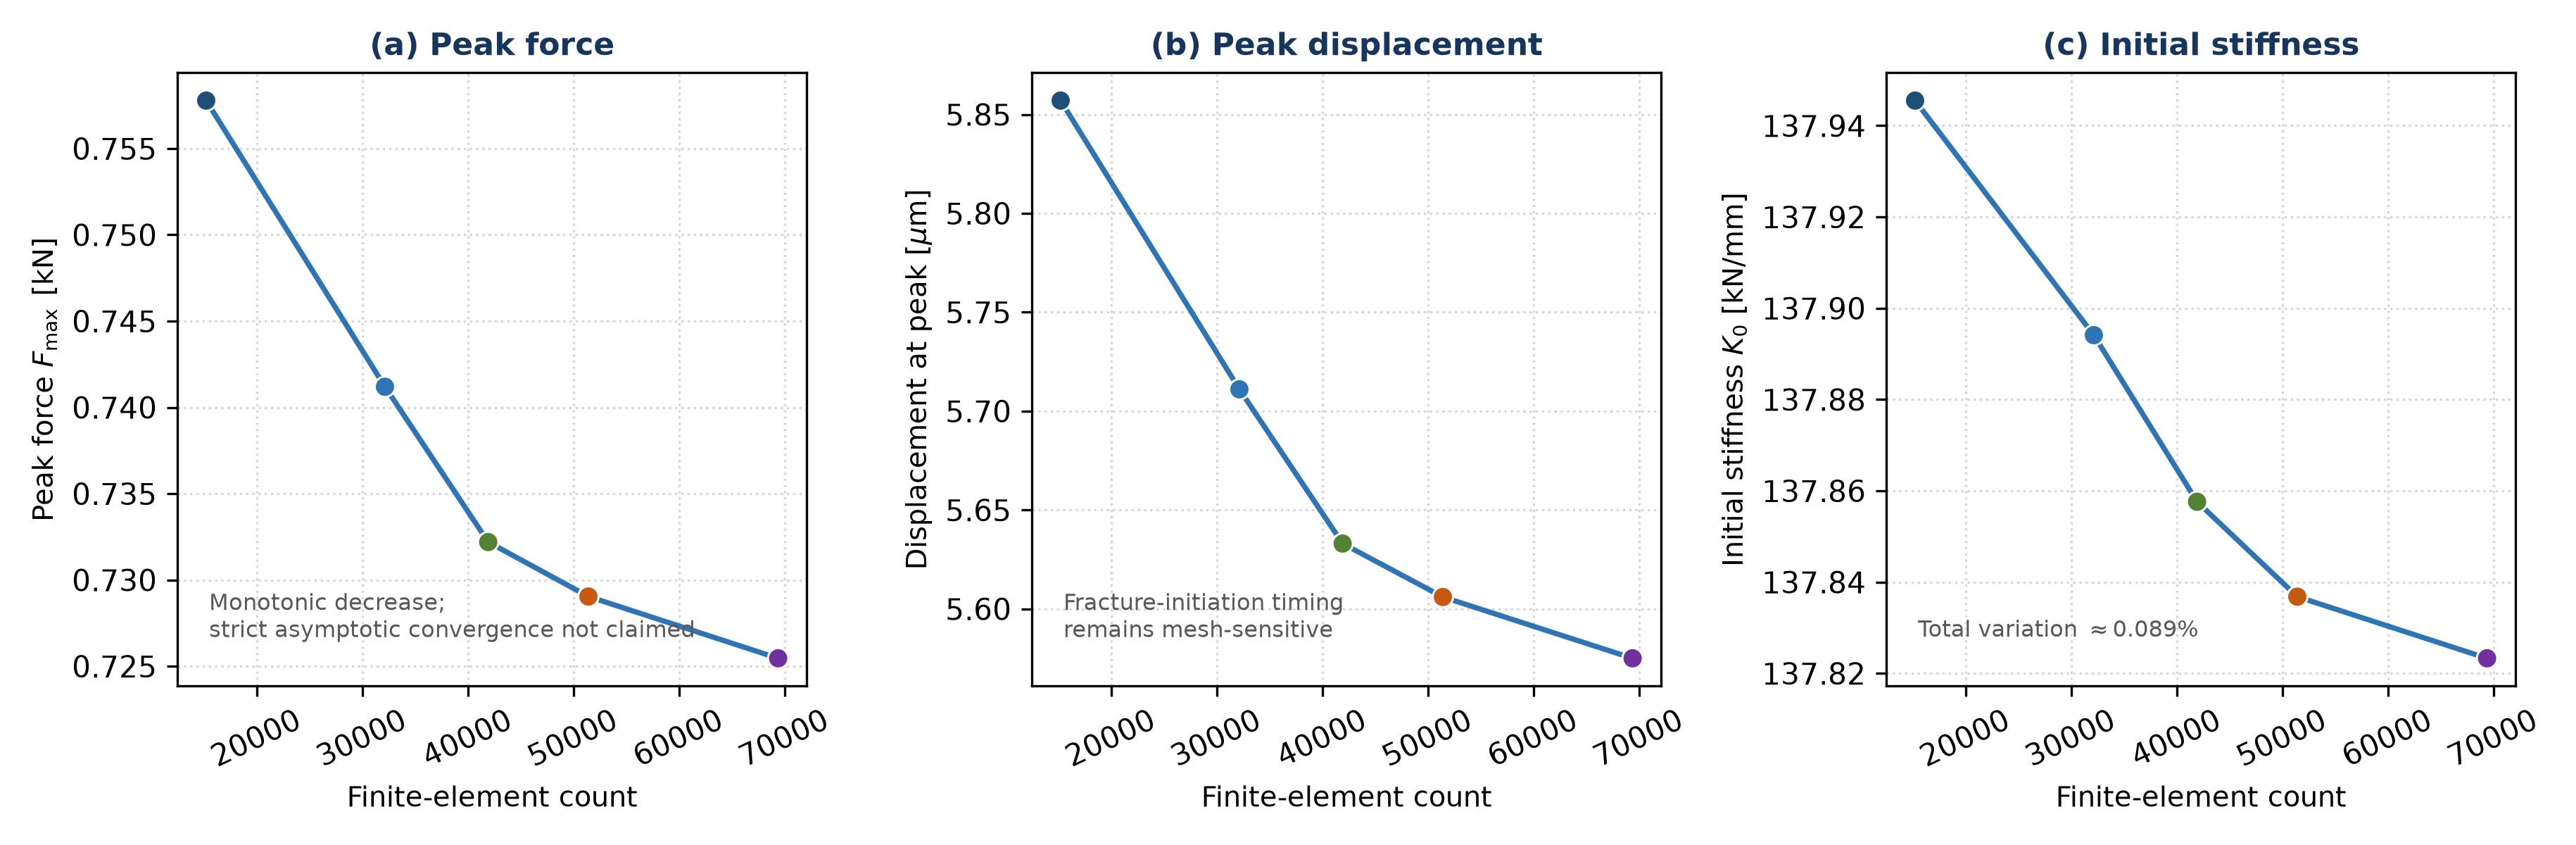
\includegraphics[width=0.96\textwidth,height=50mm,keepaspectratio]{fig_convergence_fu_overlay.png}
\caption{Verified scalar convergence metrics for the five qualified fixed meshes (Jobs 1401527, 1401528, 1401529, 1402827, and 1402828). No reconstructed force--displacement trajectories are used.}
\end{figure}
\vspace{-2mm}

{\footnotesize\textbf{Do the complete structural responses converge?} The elastic response is essentially mesh-independent over the investigated range. Peak force decreases monotonically as $0.757778 \to 0.741194 \to 0.732196 \to 0.729041 \to 0.725460$ kN, but the fracture-related response remains mesh-sensitive and strict asymptotic convergence is not established. Because raw complete $F$--$u$ histories for four refined jobs are not preserved in the report package, a defensible five-curve overlay is not shown and strict full-curve convergence is not claimed. Job \texttt{1398090} remains the named response anchor; parallel parity jobs are not double-counted in the sequence.}


\newpage
\subsection{External Work and Spatial Evidence Status}
\textbf{The quantity $W_{\mathrm{ext}}(u) = \int_0^u F(\tilde{u})\,\mathrm{d}\tilde{u}$ is the external mechanical work obtained from the global reaction-force--displacement response. It is not presented as Abaqus internal energy or fracture energy, because the present UEL does not provide a fully qualified built-in ENERGY balance.}

Because Job \texttt{1401528} ($h=0.00200$ mm) terminated automatically at $u_{\mathrm{end}} = 0.006816$ mm and Job \texttt{1402827} ($h=0.00125$ mm) at $u_{\mathrm{end}} = 0.007208$ mm, external work is evaluated over the common displacement interval $u \in [0, 0.006816\,\mathrm{mm}]$ ($u \le 6.82\,\mu\mathrm{m}$). Over this common cutoff, $W_{\mathrm{ext}}$ decreases monotonically across the five meshes from $2.3583$ to $2.1475$ mJ. Successive changes become substantially smaller at the finer levels overall, although the final change is slightly larger than the preceding one; therefore no formal asymptotic convergence order is claimed. The reference-only cutoff value of $0.00235865$ J ($2.35865$ mJ) over $u \le 0.007670$ mm applies to the reference baseline, but cannot be evaluated directly for meshes that terminated earlier.

Quantitative phase-field and crack-path values are withheld from this supervisor report because the required five-job provenance package is not preserved. Retaining numerical values would require, for every job, the actual extracted $x$--$d$ pairs, matched step/frame and displacement, crack-path coordinates, extraction settings, and the calculation used for any $L_2$ difference or characteristic front location. Until those artifacts exist, spatial convergence is evaluated qualitatively from localization around the expected $y=0.5$ mm ligament and is not assigned numerical convergence metrics.

\begin{figure}[H]
\centering
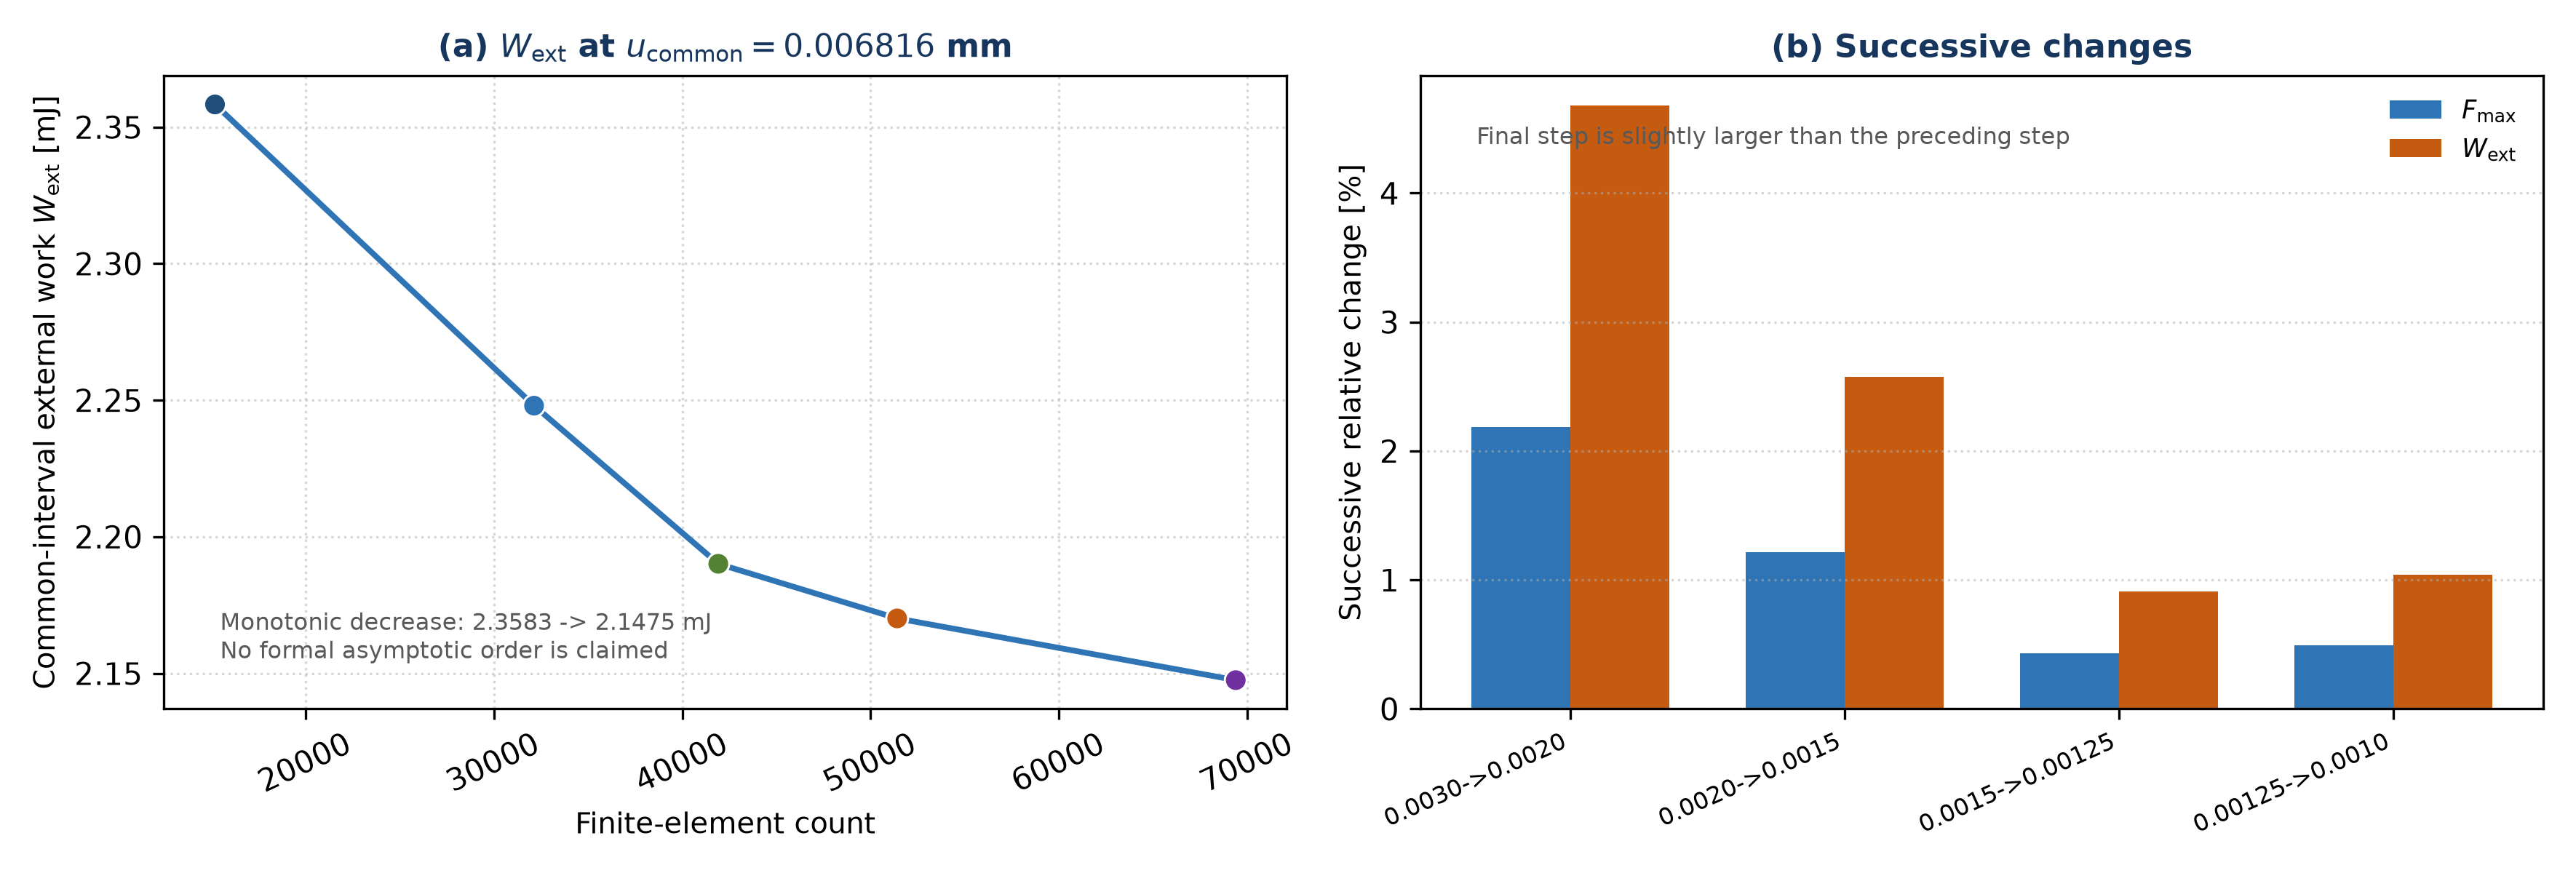
\includegraphics[width=0.96\textwidth,height=68mm,keepaspectratio]{fig_convergence_work_and_spatial.png}
\caption{Common-interval external work and successive relative changes in peak force and external work. The final refinement step is slightly larger than the preceding step, so no formal convergence order is reported.}
\end{figure}

\textbf{Multifaceted convergence assessment:} The initial elastic structural response is essentially mesh-independent, with $K_0$ varying by approximately $0.089\%$ across a $4.56$-fold increase in finite-element count. In contrast, $F_{\max}$, $u(F_{\max})$, and common-interval external work retain measurable mesh sensitivity. Strict asymptotic convergence is not claimed from the peak-load sequence. Phase-field and crack-path convergence remain required parts of mesh adequacy, but quantitative spatial conclusions are deferred until auditable five-job extraction artifacts are preserved.

\newpage
\section{Published Adaptive Workflow}
The paper describes a two-job pre-refinement process. The coarse analysis is converted to the layered UEL/facsimile representation, MISESERI is requested on \texttt{All\_elem}, and Abaqus native remeshing generates a separate refined input for the final phase-field solve.
\begin{figure}[H]
\centering
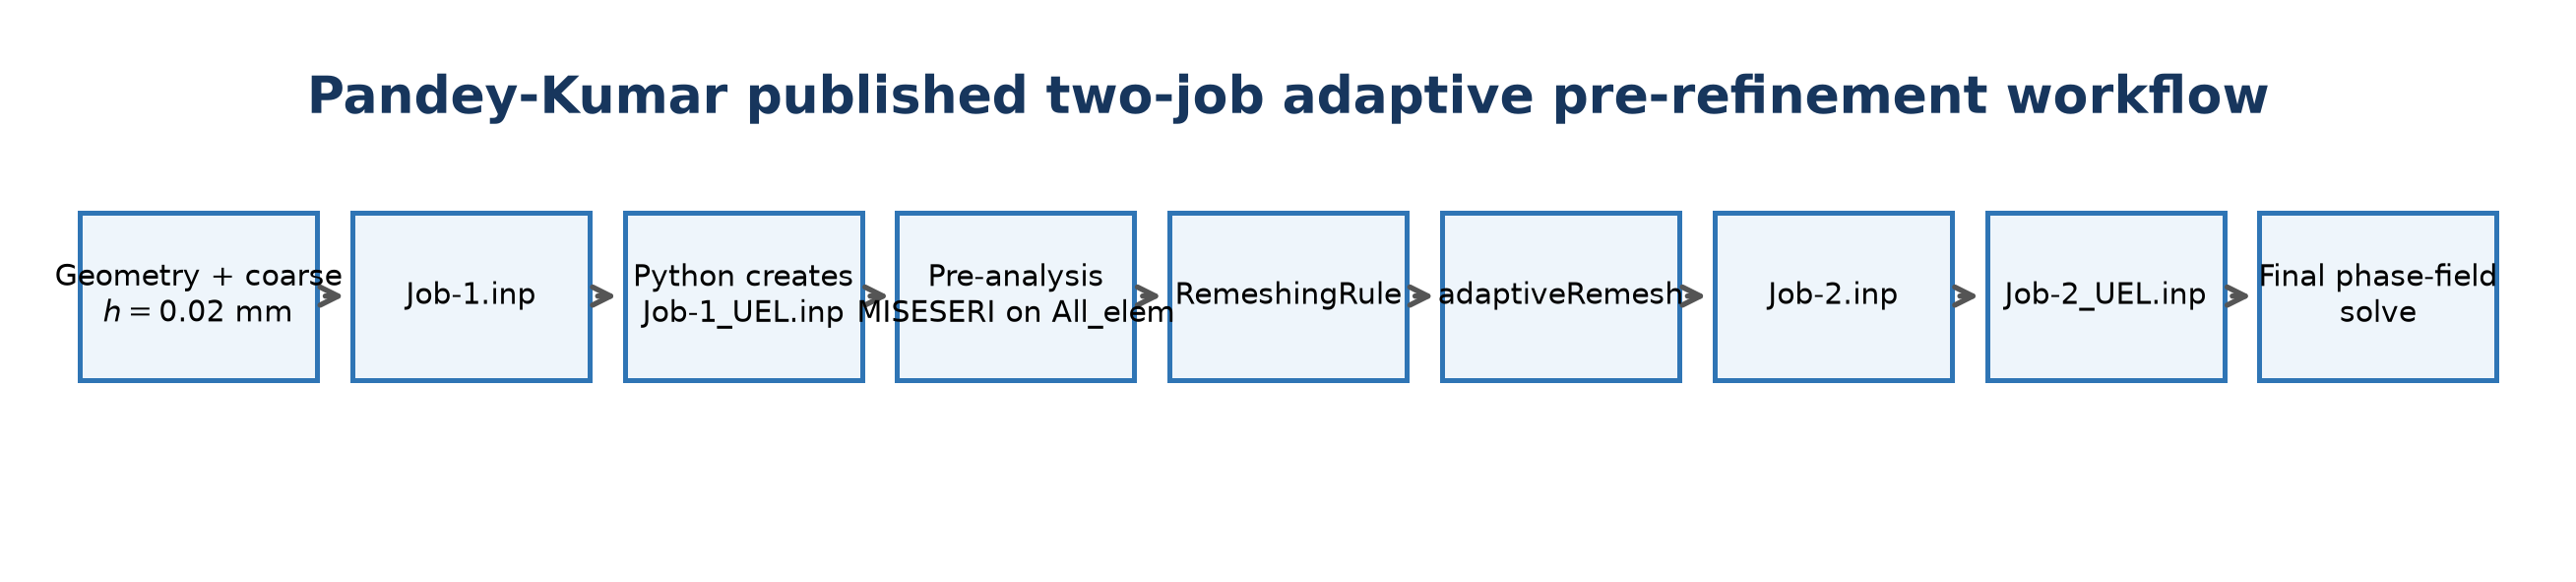
\includegraphics[width=\textwidth,height=48mm,keepaspectratio]{published_workflow.png}
\caption{Published Job-1 to Job-2 adaptive pre-refinement workflow.}
\end{figure}
\small
\par\smallskip\noindent
\begin{tabularx}{\textwidth}{>{\RaggedRight\arraybackslash}p{0.47\textwidth}>{\RaggedRight\arraybackslash}p{0.47\textwidth}}
\headrow Paper reported proposed Mode-I mesh & Project reconstruction\\
Initial global size $h=0.02$ mm\newline No local pre-refinement\newline Initial coarse count: \textbf{not reported}\newline Adaptive local size $h=0.001$ mm\newline Final adapted count: \textbf{13,941} & Initial coarse pre-analysis: \textbf{2,906 finite elements}\newline MISESERI on 2,906 underlying elements\newline \texttt{errorTarget=1.0}\newline Native \texttt{adaptiveRemesh}\newline Final adapted count: \textbf{71,320}\\
\end{tabularx}\par\smallskip
\normalsize

\textbf{The workflow is not a refinement of the 26,282-element standard-PFM mesh.} \texttt{Job-1\_UEL} belongs to the separate proposed adaptive branch, and \texttt{Job-2\_UEL} is the refined result of that branch.
\src{Pandey and Kumar (2025), Section 3.3 and Listings 1-4; project canonical pre-analysis audit.}

\newpage
\section{MISESERI and Uniform Error Sizing}
MISESERI is an Abaqus stress discretization error indicator associated with the recovered von Mises stress field. A relatively large value indicates that the local finite-element stress representation is comparatively under-resolved. Under \texttt{UNIFORM\_ERROR} sizing, such regions tend to demand a finer target mesh. Smaller-error regions demand less refinement. Because \texttt{coarseningFactor=NOT\_ALLOWED}, the present rule does not use low-error regions to coarsen the mesh.
\begin{figure}[H]
\centering
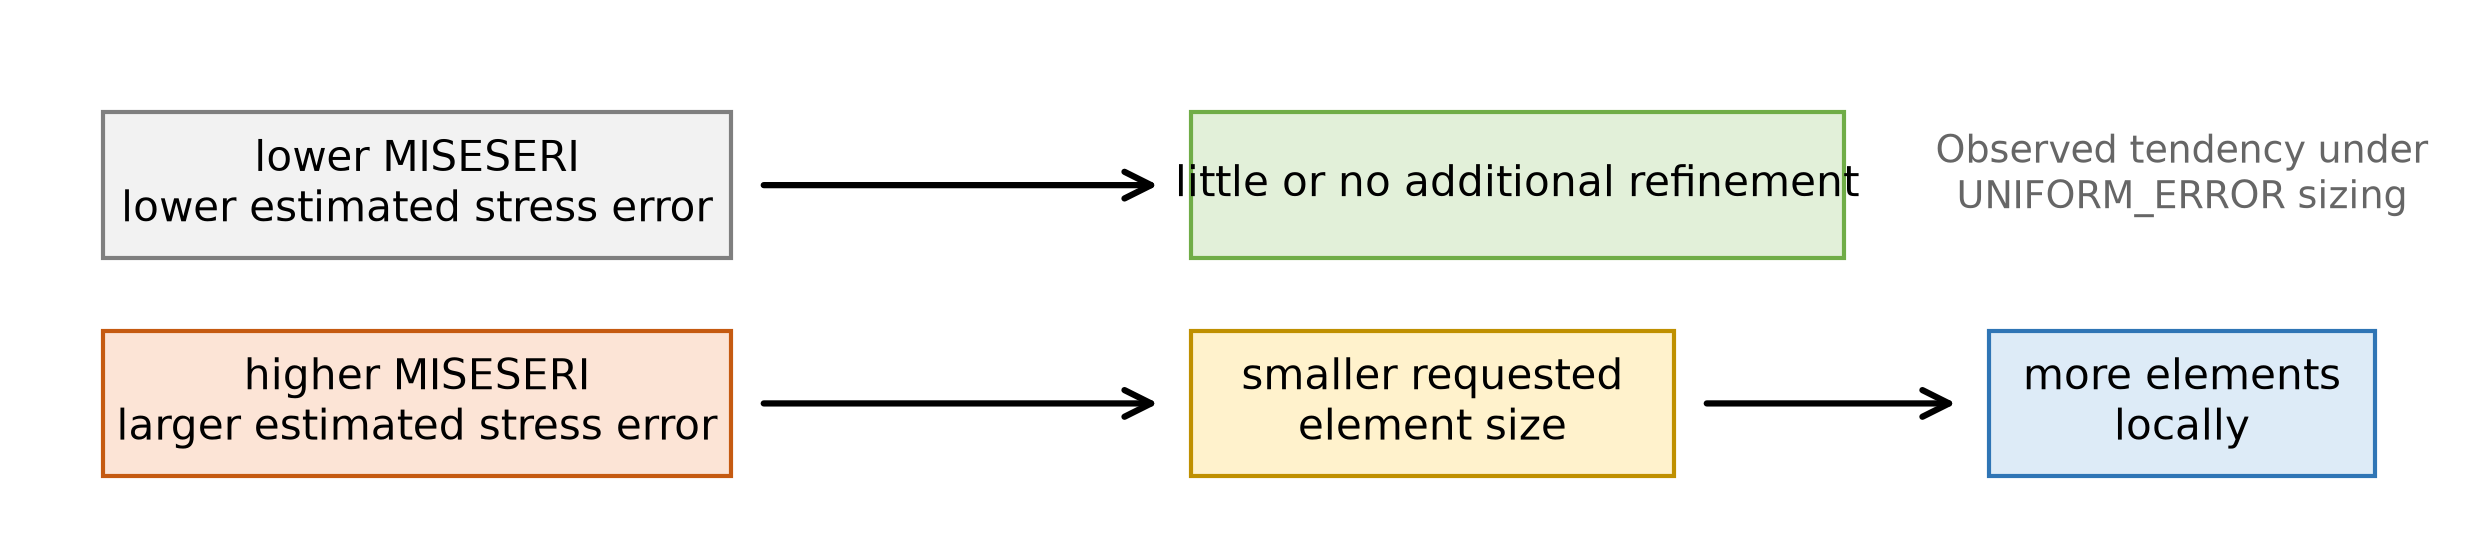
\includegraphics[width=0.94\textwidth,height=36mm,keepaspectratio]{miseseri_concept.png}
\caption{Defensible qualitative interpretation of MISESERI under the reported remeshing rule.}
\end{figure}
\vspace{-2mm}
\begin{figure}[H]
\centering
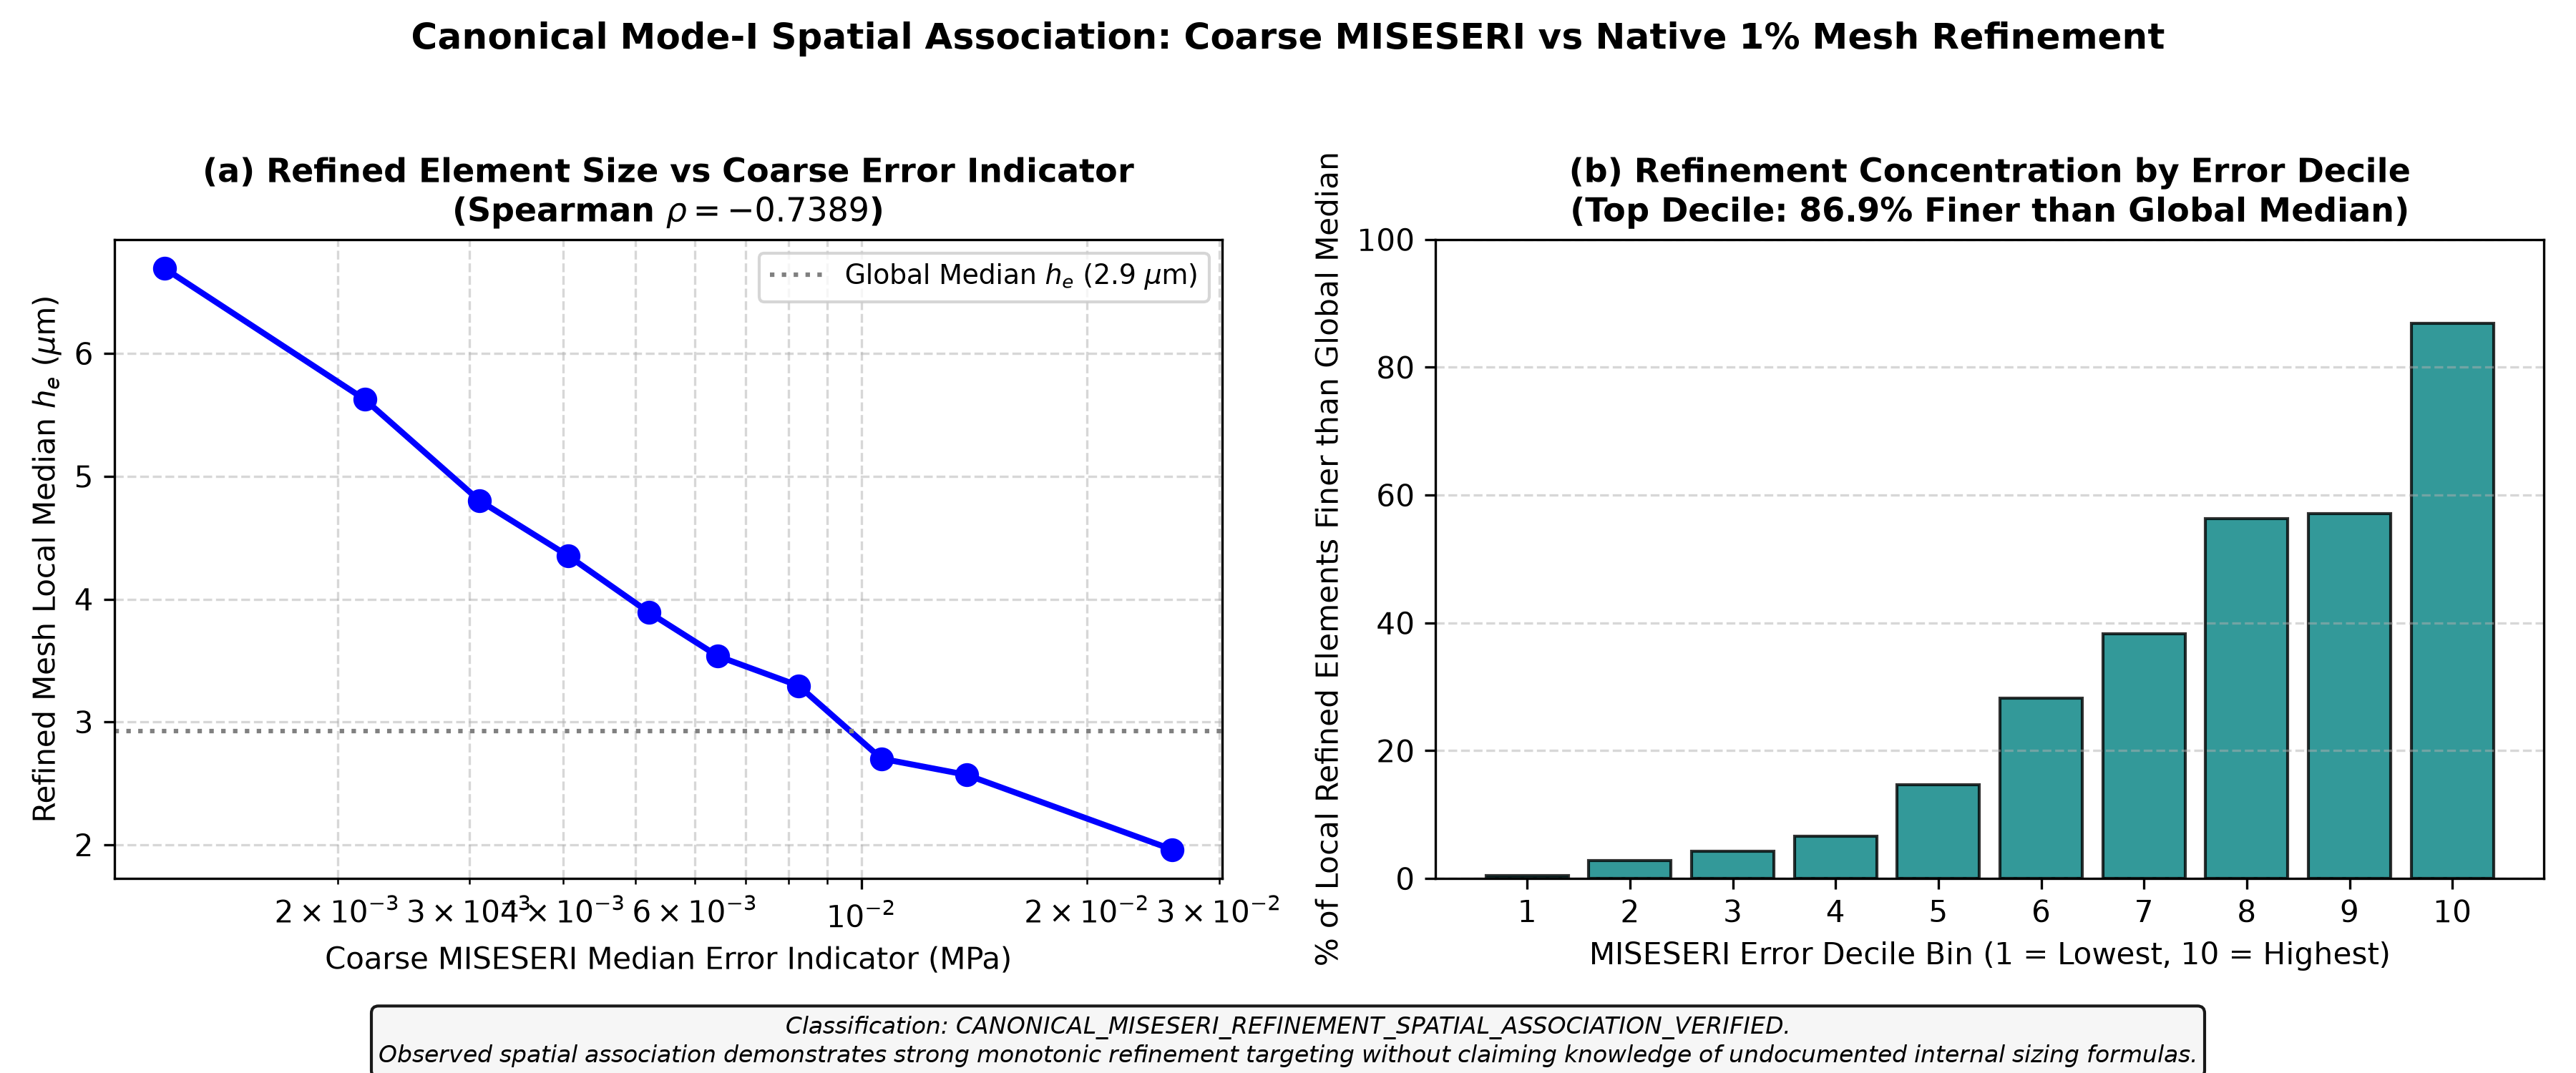
\includegraphics[width=\textwidth,height=83mm,keepaspectratio]{miseseri_spatial.png}
\caption{Observed project relationship between coarse MISESERI and local size in the native 1\% mesh. This is an empirical spatial association, not a universal sizing formula.}
\end{figure}
\vspace{-2mm}
{\small\texttt{errorTarget=1.0} specifies a \textbf{1\% target error tolerance under Abaqus UNIFORM\_ERROR sizing}. It does not mean ``refine 1\% of the elements,'' and it is not the direct condition \texttt{MISESERI >= 0.01}. Abaqus combines the error field, target tolerance, size bounds, refinement factor and internal sizing logic. The exact internal MISESERI-to-$h$ transformation has not been established from the available documentation or evidence.}

\newpage
\section{Stiffness Anomaly and Boundary Set Repair}
The low-stiffness 71,320-element branch was caused by malformed \texttt{N\_BOTTOM} formatting, not by the adaptive mesh or phase-field constitutive response. The original set placed 150 node IDs on one free-format data line; Abaqus retained only the first 16, leaving 134 bottom nodes free vertically.
\begin{figure}[H]
\centering
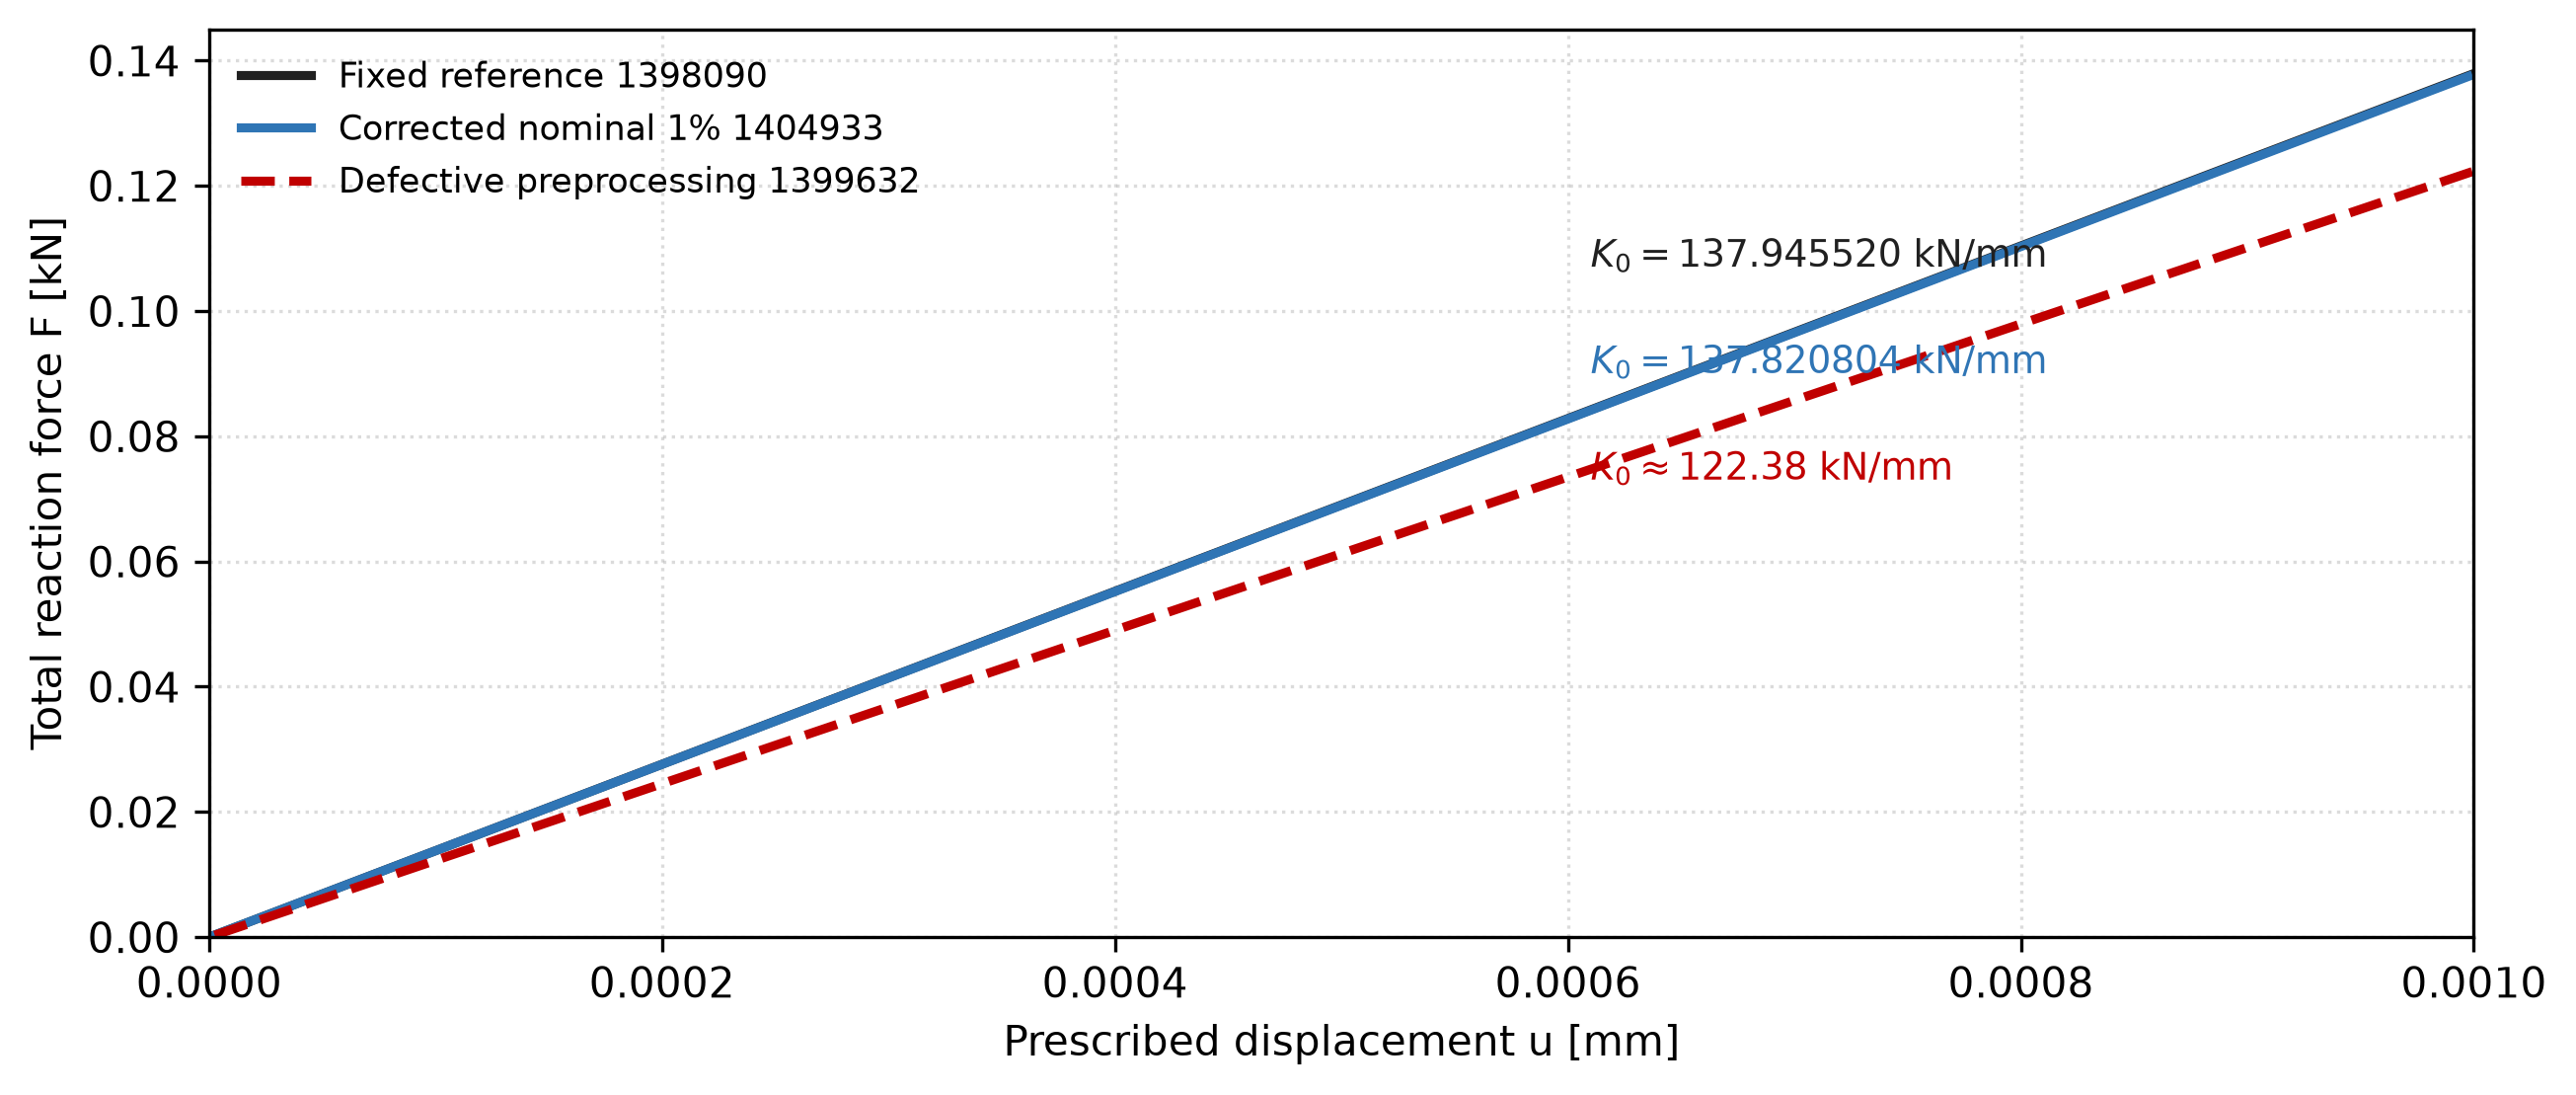
\includegraphics[width=0.96\textwidth,height=75mm,keepaspectratio]{force_displacement_zoom.png}
\caption{Initial elastic-range zoom. The corrected model and fixed reference overlap near 138 kN/mm; the defective branch remains near 122.38 kN/mm.}
\end{figure}
\vspace{-2mm}
\begin{figure}[H]
\centering
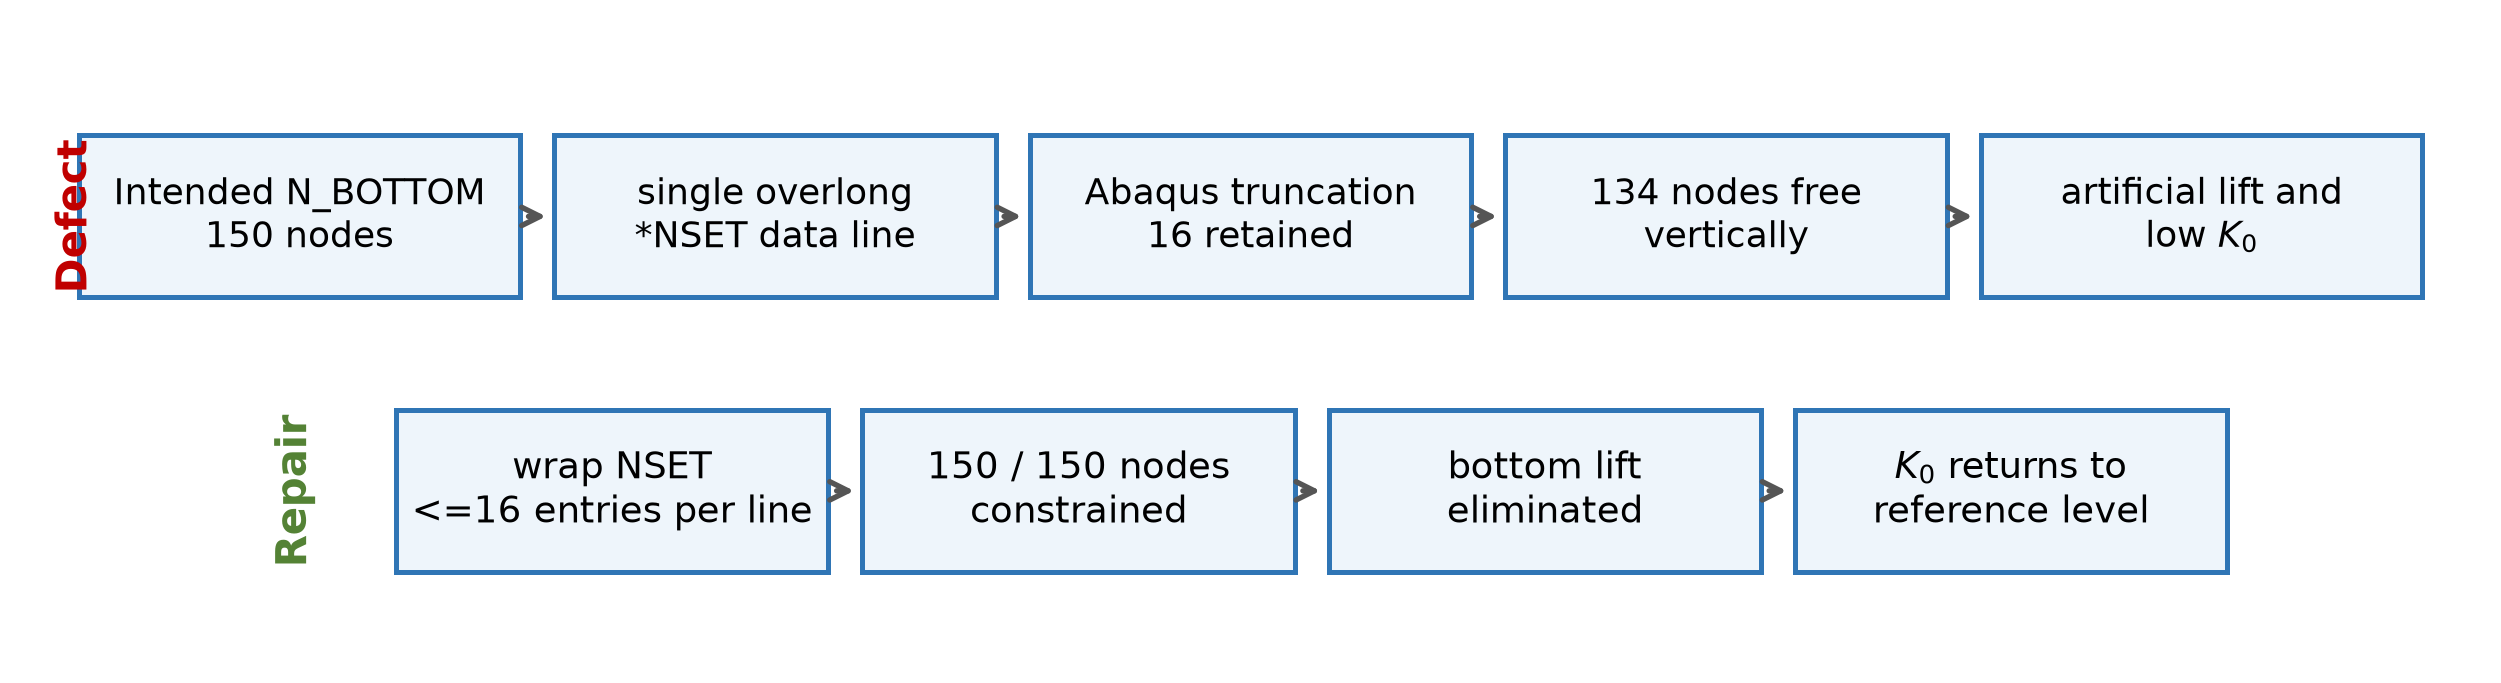
\includegraphics[width=0.96\textwidth,height=50mm,keepaspectratio]{boundary_set_flow.png}
\caption{Verified preprocessing defect and deterministic repair.}
\end{figure}
\vspace{-1mm}
\scriptsize
\par\smallskip\noindent
\begin{tabularx}{\textwidth}{>{\bfseries}Yrrrr}
\headrow Model & Elements & $K_0$ [kN/mm] & $F_{\max}$ [kN] & $u(F_{\max})$ [mm]\\
Fixed reference 1398090 & 15,192 & 137.945520 & 0.757778 & 0.005857\\
\rowcolor{paleblue}Defective diagnostic 1399632 & 71,320 & about 122.38 & 0.478203 & 0.004150\\
Corrected nominal 1\% 1404933 & 71,320 & 137.820804 & 0.745325 & 0.005750\\
\end{tabularx}\par\smallskip
\normalsize
{\small A separate frozen-damage requalification, Job 1405044, independently recovered $K_0=138.021013$ kN/mm, confirming that stiffness recovery occurs before fracture evolution.}

\newpage
\section{Abaqus Release Study}
The canonical native remeshing operation was reproduced across the installed Linux releases. The generated adapted topology remained unchanged, so release version does not explain the 71,320-versus-13,941 discrepancy.
\small
\par\smallskip\noindent
\begin{tabularx}{\textwidth}{>{\bfseries}p{45mm}p{38mm}Y}
\headrow Abaqus environment & Adapted finite elements & Result\\
Abaqus 2019 Linux & 71,320 & same canonical adapted topology/artifact\\
\rowcolor{paleblue}Abaqus 2021 Linux & 71,320 & same\\
Abaqus 2022 Linux & 71,320 & same\\
\rowcolor{paleblue}Abaqus 2023 Linux & 71,320 & same\\
\end{tabularx}\par\smallskip
\normalsize

\textbf{Within the tested Linux Abaqus 2019-2023 releases, release version does not explain the 71,320-versus-13,941 discrepancy.}

The Abaqus 2019 PBS wrapper had a walltime/logging issue, but the generated remeshing artifact was available and matched the canonical result. Any Windows/Abaqus 2024 observation should be treated separately as a platform-plus-release-confounded sensitivity, not as a clean release comparison.

\subsection{What the release result rules out}
\begin{itemize}
\item A simple Linux release change from 2019 through 2023 does not change the adapted count.
\item The element-count discrepancy therefore requires a different explanation, such as an unreported modeling, meshing or execution detail.
\item This conclusion concerns the generated adaptive mesh artifact; it does not claim identity of every solver or scheduler detail.
\end{itemize}

\newpage
\section{Standard PFM versus Proposed Adaptive PFM versus This Reconstruction}
All three lanes address the same Mode-I benchmark, but they are independent discretization strategies. The two paper counts are final counts from different simulations, while the project count pair explicitly shows the before-and-after values within one adaptive route.
\begin{figure}[H]
\centering
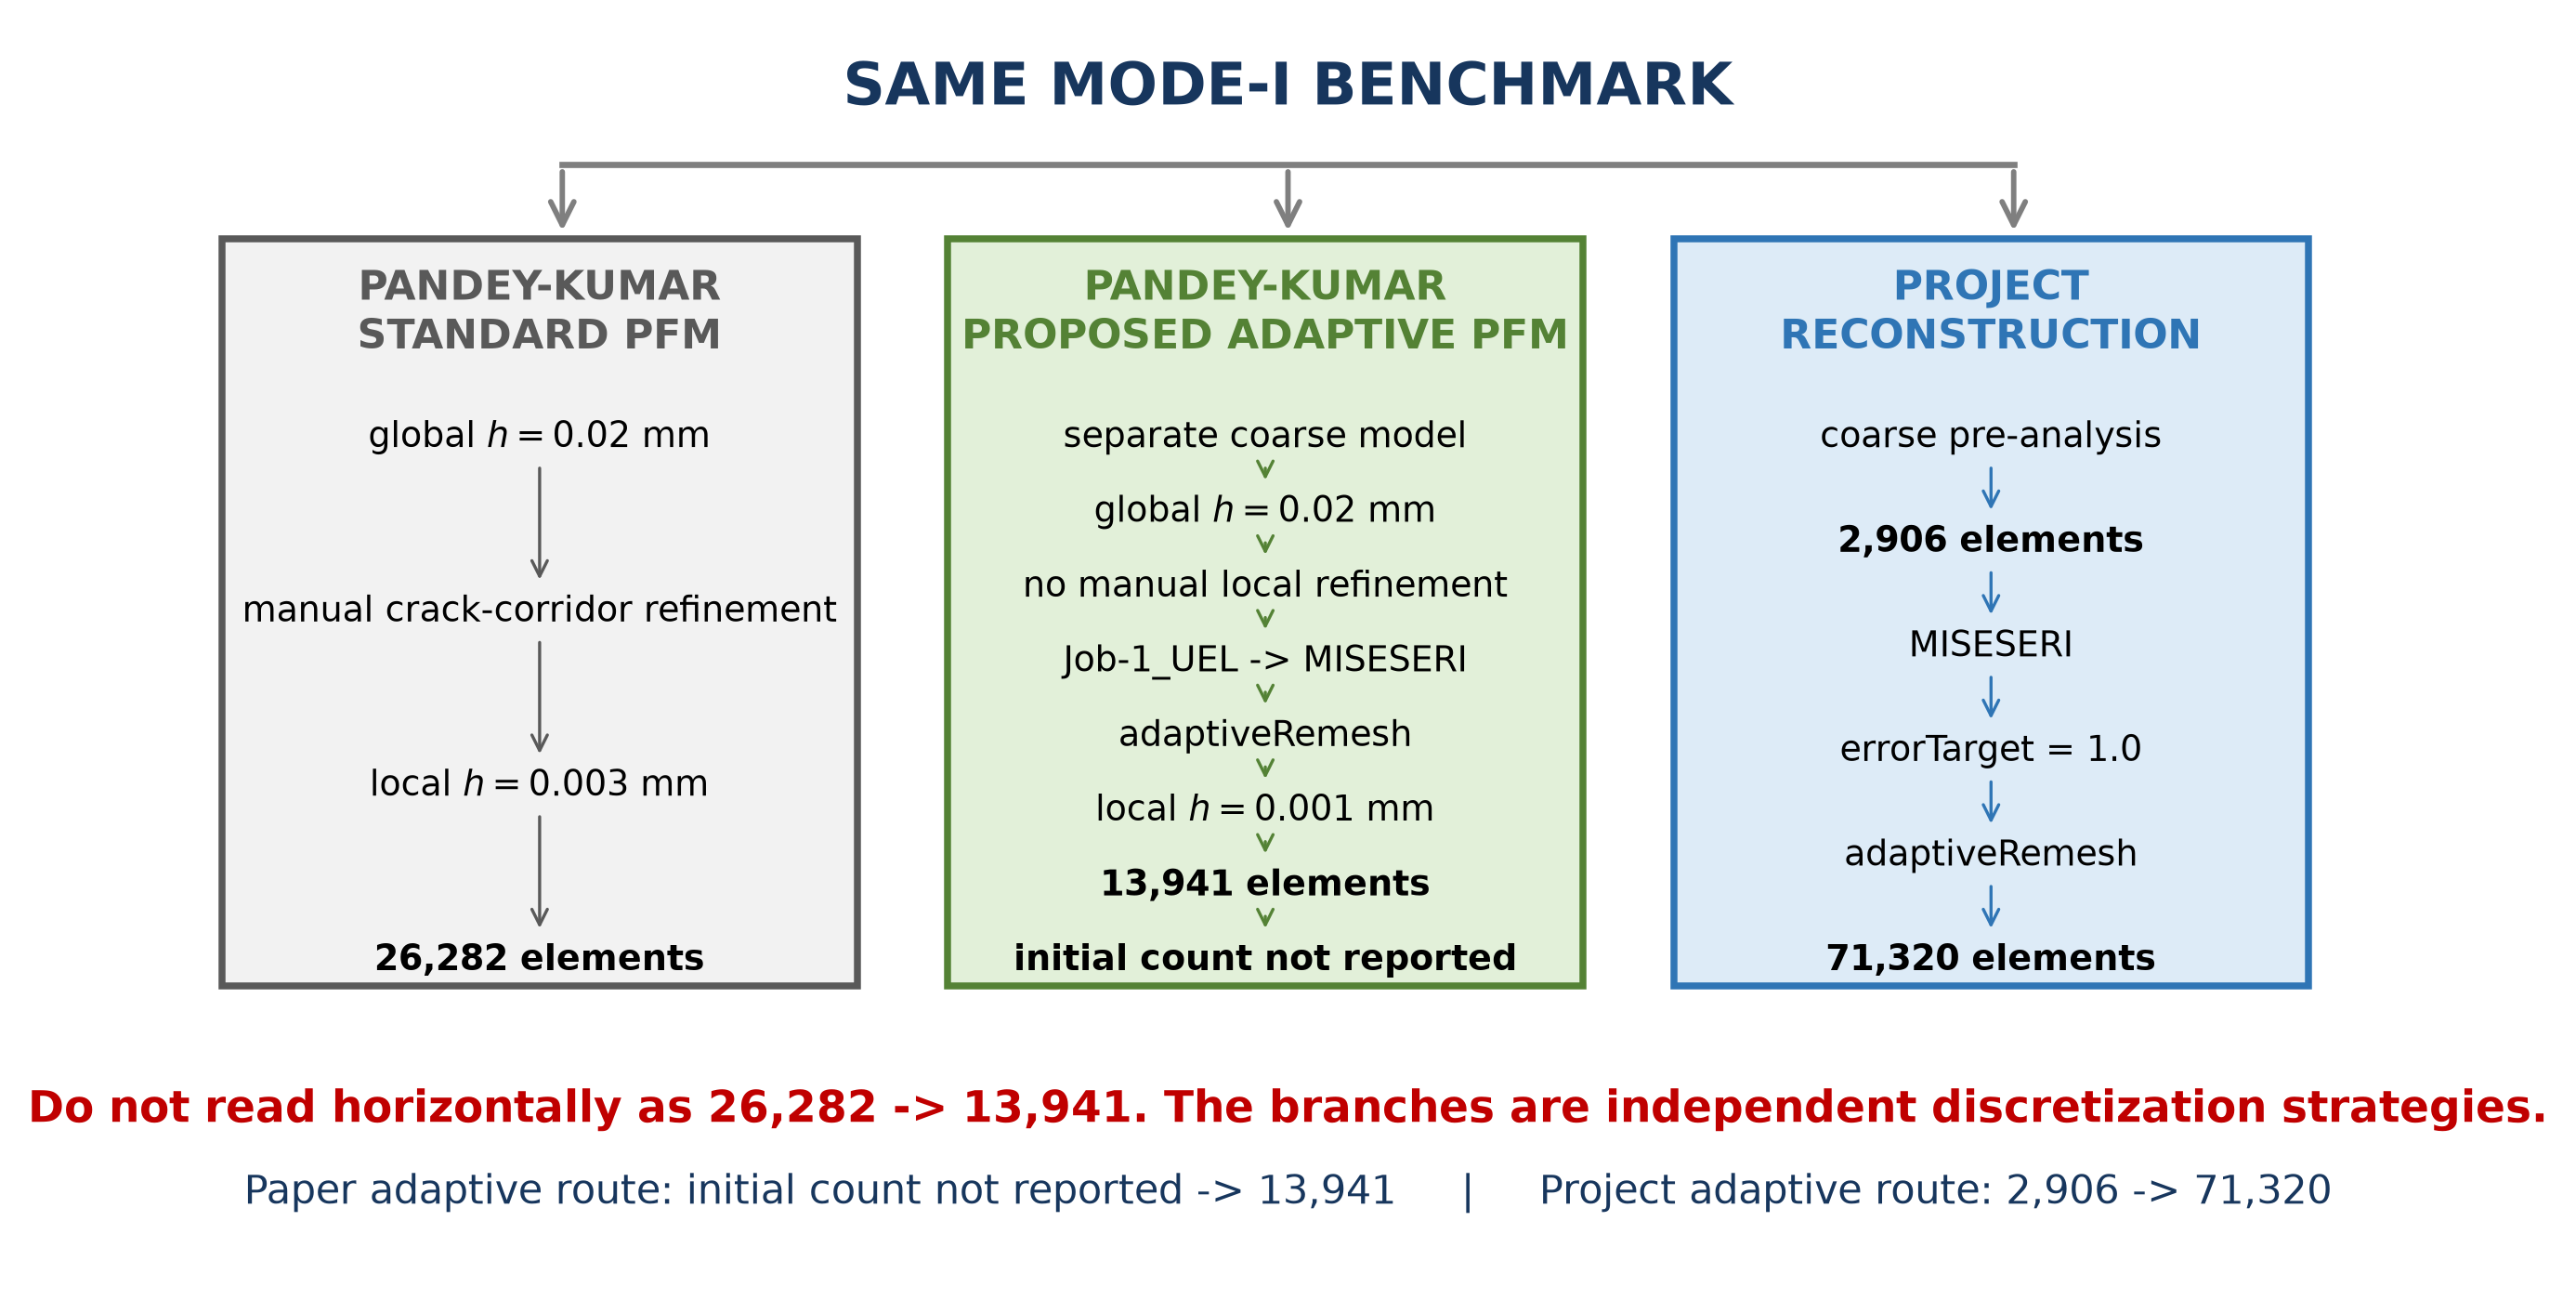
\includegraphics[width=\textwidth,height=150mm,keepaspectratio]{three_branch_mesh_routes.png}
\caption{Independent meshing branches and the only valid within-route count comparisons.}
\end{figure}
\vspace{-2mm}
\textbf{\color{rednote}Do not read this figure horizontally as 26,282 $\rightarrow$ 13,941. The branches are independent discretization strategies.}

\textbf{Paper adaptive route: initial count not reported $\rightarrow$ 13,941.}\quad \textbf{Project adaptive route: 2,906 $\rightarrow$ 71,320.}

{\small Abaqus uses MISESERI and the \texttt{RemeshingRule} settings to determine a spatial target-size field. The inputs and resulting mesh are observable, but the exact internal numerical transformation has not been established. The report therefore compares verified input fields, rule parameters, spatial patterns and resulting element counts rather than inventing a direct MISESERI-to-$h$ equation.}

\newpage
\section{Element Count Discrepancy Sensitivity Audit}
{\small The following one-factor tests show how the adapted count responds to controlled changes. Several factors materially change the count, but none reproduces 13,941 while retaining the published Mode-I \texttt{RemeshingRule} settings.}
\scriptsize
\renewcommand{\arraystretch}{1.15}
\par\smallskip\noindent
\begin{tabularx}{\textwidth}{>{\RaggedRight\arraybackslash\bfseries}p{62mm}>{\centering\arraybackslash}p{31mm}Y}
\headrow One-factor test & Adapted finite elements & Interpretation\\
Canonical \texttt{errorTarget=1.0} & 71,320 & baseline\\
\rowcolor{paleblue}Abaqus 2019 Linux & 71,320 & release insufficient\\
Abaqus 2021 Linux & 71,320 & release insufficient\\
\rowcolor{paleblue}Abaqus 2022 Linux & 71,320 & release insufficient\\
Abaqus 2023 Linux & 71,320 & release insufficient\\
\rowcolor{paleblue}\texttt{outputFrequency=LAST\_INCREMENT} & 71,320 & no effect\\
\texttt{refinementFactor=3} & 47,428 & substantial effect; insufficient\\
\rowcolor{paleblue}coarsening enabled/default & 71,037 & negligible\\
minimum-size specification removed & 71,320 & no effect\\
\rowcolor{paleblue}maximum-size specification removed & 70,736 & negligible\\
coarse global seed 0.03 mm & 48,919 & substantial but insufficient\\
\rowcolor{paleblue}top-edge $U_1$ released & 55,761 & substantial but insufficient\\
CPE4 $\rightarrow$ CPE4R & 103,706 & wrong direction\\
\rowcolor{paleblue}CPS4 branch & 58,679 & confounded formulation sensitivity\\
\texttt{errorTarget=2.0} & 17,687 & sensitivity only; not evidence paper used 2\%\\
\rowcolor{paleblue}\texttt{errorTarget=3.0} & 8,120 & sensitivity only\\
\texttt{errorTarget=5.0} & 4,356 & sensitivity only\\
\end{tabularx}\par\smallskip
\normalsize
\renewcommand{\arraystretch}{1}

{\small Element-count proximity alone cannot identify the paper's executed setting. In particular, the 2\%, 3\% and 5\% branches are sensitivity results; they do not show that Pandey and Kumar used a different \texttt{errorTarget} from the published value of 1.0.}

\newpage
\section{Remaining Mode I Discrepancy and Current Scientific Conclusion}
The canonical reconstruction produces 71,320 finite elements whereas Pandey and Kumar report 13,941 for their proposed Mode-I adaptive mesh. Abaqus release, output frequency, top lateral constraint, element formulation, global seed, coarsening, refinement factor, sizing bounds and error-target sensitivities have been investigated. Several parameters materially change the mesh count, but no tested case reproduces 13,941 while simultaneously preserving the retained published Mode-I \texttt{RemeshingRule} settings. The exact source of the discrepancy therefore remains unresolved.

\subsection{Conclusions}
\begin{itemize}
\item The fixed reference reproduces the published Mode-I force-displacement response closely.
\item The paper's 26,282-element standard mesh and 13,941-element adaptive mesh are separate branches, not the before-and-after states of one remeshing operation.
\item The low-stiffness 71,320 branch was caused by malformed \texttt{N\_BOTTOM} formatting and is resolved.
\item The corrected 71,320-element model recovers $K_0$ but retains a modest peak-response difference.
\item Canonical 1\% native remeshing gives 71,320 finite elements versus the paper's 13,941.
\item Abaqus 2019-2023 does not explain the discrepancy.
\item Multiple controlled sensitivities alter the adapted count but do not establish the reported 13,941 configuration.
\item The remaining element-count discrepancy is the unresolved Mode-I reproduction question.
\end{itemize}

\small
\par\smallskip\noindent
\begin{tabularx}{\textwidth}{>{\bfseries}Yp{50mm}p{42mm}}
\headrow Comparison & Initial adaptive-branch count & Final adapted count\\
Pandey-Kumar adaptive route & not reported & 13,941\\
\rowcolor{paleblue}Project adaptive route & 2,906 & 71,320\\
\end{tabularx}\par\smallskip
\normalsize

\newpage
\section{References}
\begin{enumerate}[leftmargin=7mm,itemsep=6pt]
\item Pandey, A. and Kumar, S. (2025). A Simple and Robust Mesh Refinement Implementation in Abaqus for Phase Field Modelling of Brittle Fracture. \textit{Computer Modeling in Engineering and Sciences}, 144(3), 3251-3286. \url{https://doi.org/10.32604/cmes.2025.067858}.
\item Molnar, G. and Gravouil, A. (2017). 2D and 3D Abaqus implementation of a robust staggered phase-field solution for modeling brittle fracture. \textit{Finite Elements in Analysis and Design}, 130, 27-38. \url{https://doi.org/10.1016/j.finel.2017.03.002}.
\item Msekh, M. A., Sargado, J. M., Jamshidian, M., Areias, P. M. and Rabczuk, T. (2015). Abaqus implementation of phase-field model for brittle fracture. \textit{Computational Materials Science}, 96, 472-484. \url{https://doi.org/10.1016/j.commatsci.2014.05.071}.
\item Dassault Systemes. Abaqus 2023 Documentation. Analysis User's Guide, Theory Guide and input syntax documentation for adaptive remeshing and stress error indicators.
\end{enumerate}

\subsection{Primary Project Evidence}
\begin{itemize}
\item Job 1398090 fixed response anchor and project OLS stiffness extraction.
\item Job 1399632 defective preprocessing diagnostic and \texttt{N\_BOTTOM} warning evidence.
\item Job 1404933 corrected nominal-1\% full-fracture response.
\item Job 1405044 frozen-damage stiffness requalification.
\item Canonical 2,906-element MISESERI pre-analysis and native 71,320-element adapted artifact.
\item Controlled Abaqus 2019-2023 release study and one-factor mesh-count sensitivity records.
\end{itemize}

{\small All job identifiers and numerical values in this report refer to project-controlled extraction artifacts. No element count, stiffness value or internal Abaqus sizing law has been inferred beyond the recorded evidence.}
\end{document}
